\setauthor{\secondauthor}
\subsection{Strukturierung der Fächer und Themenpools}
\label{sec:maturaupload-faecher-themenpools}

Über den Menüpunkt „Maturavorbereitung“ in der Navigationsleiste gelangen die
Nutzer:innen zur Fachauswahl. Diese Ansicht stellt den zentralen Einstiegspunkt
für die Arbeit mit Mitschriften und Fragen dar. Abhängig von der jeweiligen
Nutzerrolle unterscheidet sich die zur Verfügung stehende Funktionalität.

Das Fächer- und Themenpool-System bildet das strukturelle Grundgerüst der
Plattform. Jede Mitschrift sowie jede Frage wird eindeutig einem Fach und einem
Themenpool zugeordnet. Dadurch entsteht eine klare inhaltliche Struktur, welche
die Navigation innerhalb der Plattform sowie die Verwaltung der Inhalte
erheblich erleichtert.

\subsubsection{Fachauswahl}

\begin{figure}[h t]
    \centering
    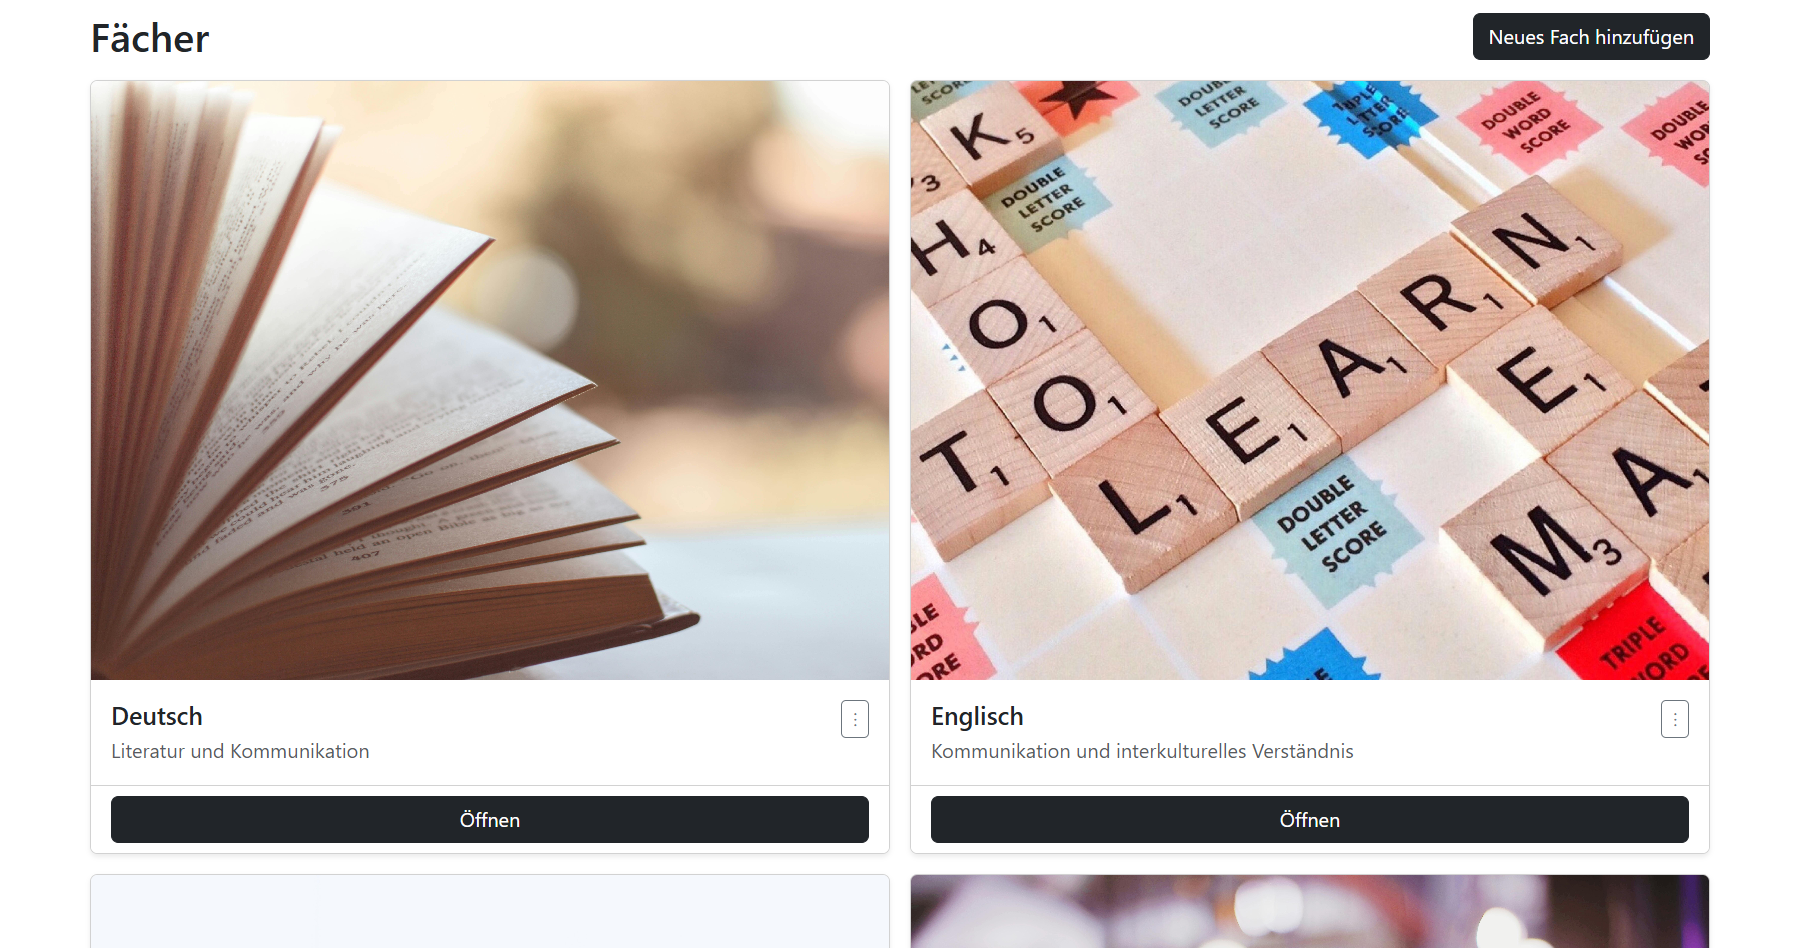
\includegraphics[width=0.7\textwidth]{pics/ab1.png}
    \caption{Fachauswahl in der Maturavorbereitung}
\end{figure}

Ein Fach stellt die oberste Ebene der inhaltlichen Organisation dar und kann
mehrere Themenpools enthalten. Die Fachauswahl ist für alle Nutzer:innen
zugänglich, unterscheidet sich jedoch je nach Rolle im dargestellten Umfang
sowie in den verfügbaren Aktionen.

\paragraph{Ansicht als Schüler:in}

Schüler:innen sehen ausschließlich jene Fächer, die bereits von Lehrkräften oder
Administrator:innen erstellt wurden. Die Fachauswahl dient in dieser Rolle
ausschließlich der Navigation und dem Zugriff auf Lernmaterialien. Funktionen
zur Erstellung, Bearbeitung oder Löschung von Fächern stehen Schüler:innen nicht
zur Verfügung.

\begin{figure}[H]
    \centering
    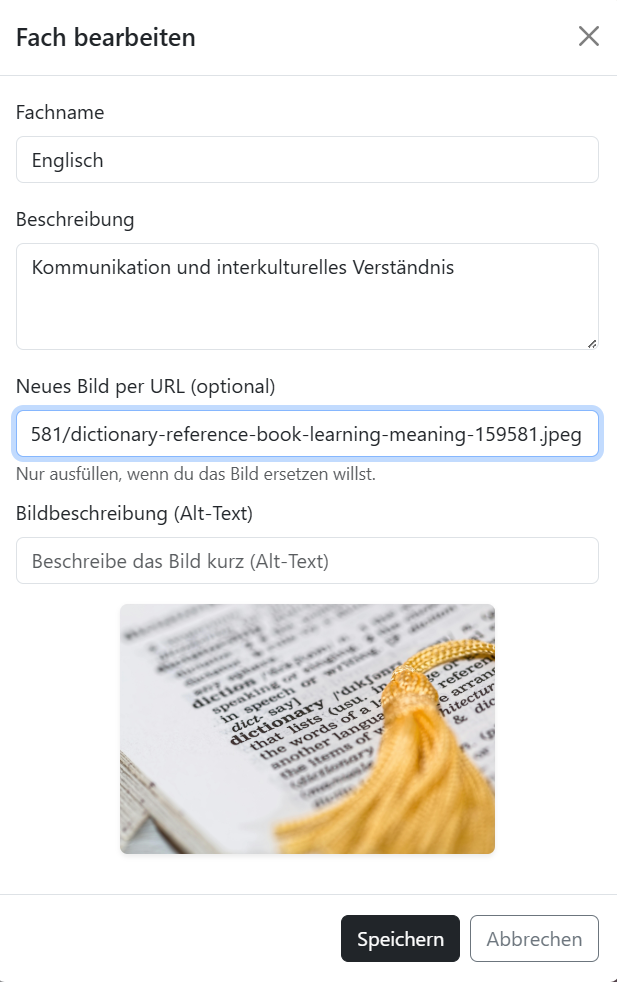
\includegraphics[width=0.7\textwidth]{pics/ab2.png}
    \caption{Fachübersicht mit erweiterten Verwaltungsfunktionen}
\end{figure}

\paragraph{Ansicht als Lehrkraft und Administrator:in}

Lehrkräfte und Administrator:innen sehen alle vorhandenen Fächer. Beide Rollen
verfügen über identische Berechtigungen in dieser Ansicht. Sie können neue Fächer
erstellen sowie bestehende Fächer bearbeiten oder löschen. Zusätzlich können
Mitschriften gezielt einem Fach zugeordnet und strukturiert verwaltet werden.

\subsubsection{Themenpool-Auswahl}

\begin{figure}[H]
    \centering
    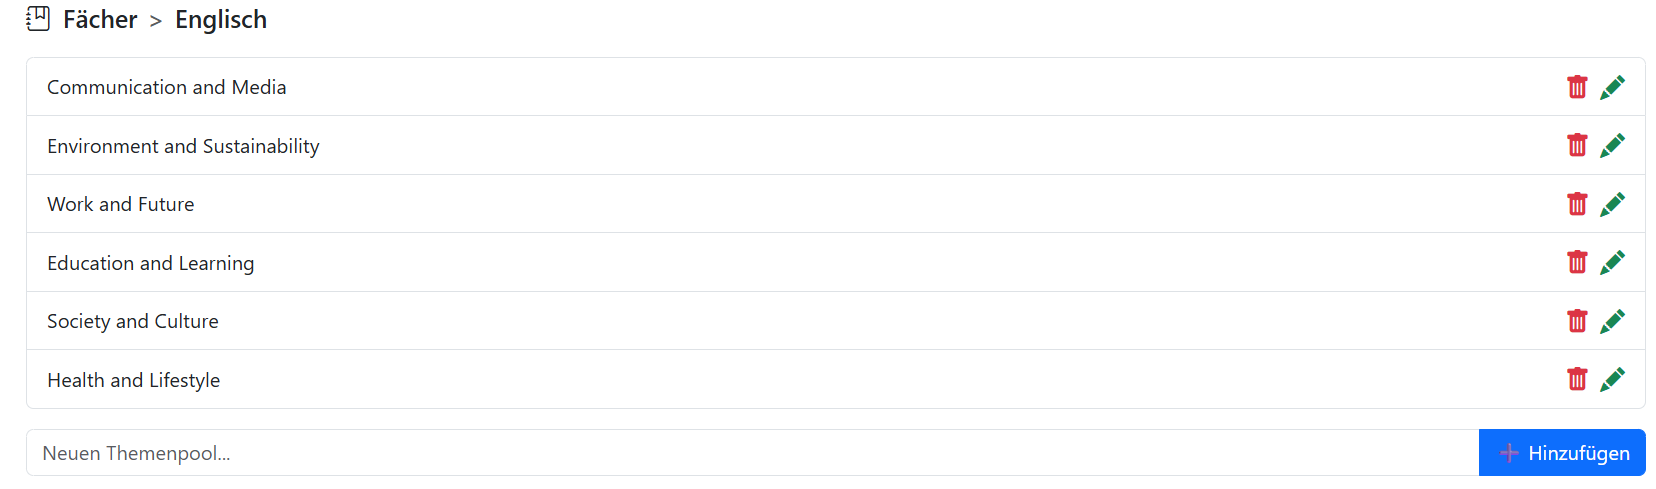
\includegraphics[width=0.7\textwidth]{pics/ab3.png}
    \caption{Themenpools innerhalb eines Faches}
\end{figure}

Themenpools bilden die zweite Ebene der inhaltlichen Struktur und dienen als
Unterkategorien eines Faches, beispielsweise \textit{Qualitätssicherung} oder
\textit{Kontrolle und Steuerung}. Jeder Themenpool ist eindeutig einem Fach
zugeordnet und enthält die zugehörigen Mitschriften.

Beim Wechsel des ausgewählten Faches werden die zugehörigen Themenpools
automatisch aktualisiert, wodurch eine konsistente und intuitive Navigation
gewährleistet wird.

\paragraph{Ansicht als Schüler:in}

Schüler:innen können Themenpools ausschließlich einsehen und zur Auswahl von
Lernmaterialien verwenden. Die Themenpool-Auswahl dient in dieser Rolle nur der
Navigation. Funktionen zur Erstellung, Bearbeitung oder Löschung von
Themenpools stehen Schüler:innen nicht zur Verfügung.

\paragraph{Ansicht als Lehrkraft und Administrator:in}

Lehrkräfte und Administrator:innen verfügen auch bei Themenpools über identische
Berechtigungen. Sie können neue Themenpools erstellen sowie bestehende
Themenpools bearbeiten oder löschen. Dadurch ist es möglich, neue inhaltliche
Bereiche anzulegen oder bestehende Strukturen flexibel anzupassen.

\subsubsection{Upload von Mitschriften}

\begin{figure}[H]
    \centering
    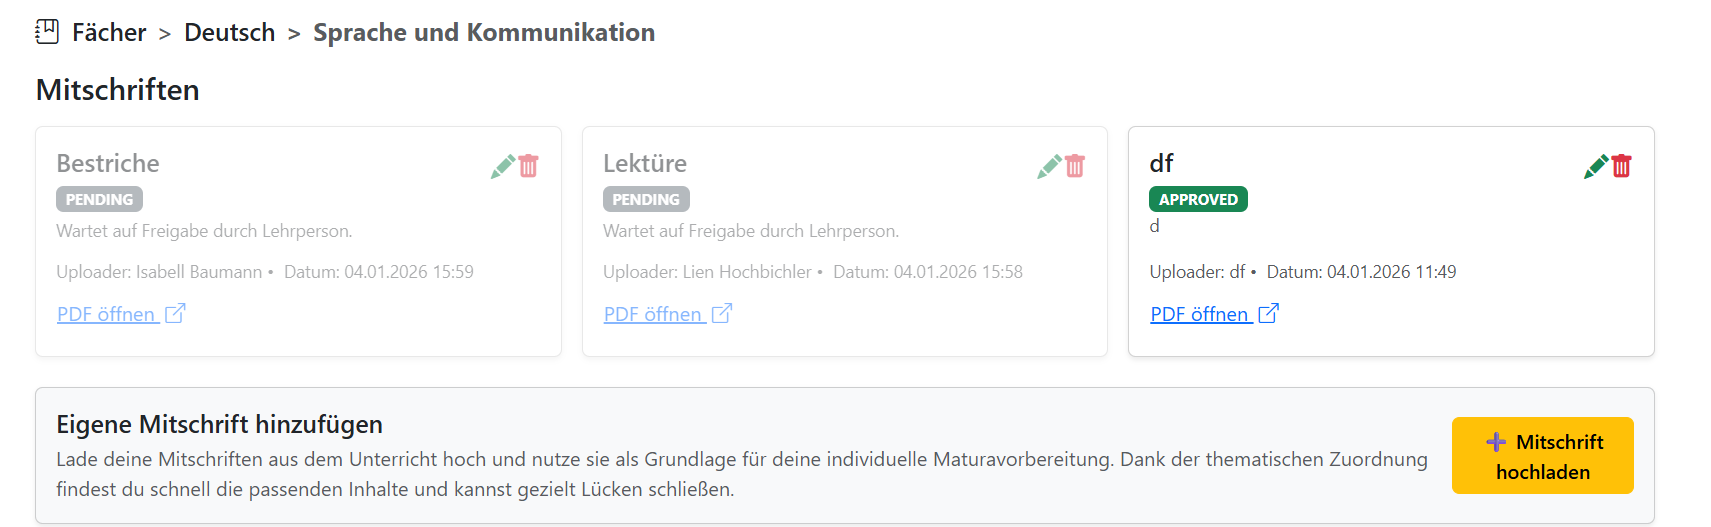
\includegraphics[width=0.7\textwidth]{pics/ab4.png}
    \caption{Mitschriftenübersicht}
    \label{fig:mitschriften}
\end{figure}

Die Plattform ermöglicht es Nutzer:innen, Mitschriften hochzuladen und diese
einem bestimmten Fach sowie einem zugehörigen Themenpool zuzuordnen. Beim Upload
müssen ein Titel sowie eine Beschreibung angegeben werden, um den Inhalt der
Mitschrift eindeutig zu kennzeichnen.

\begin{figure}[H]
    \centering
    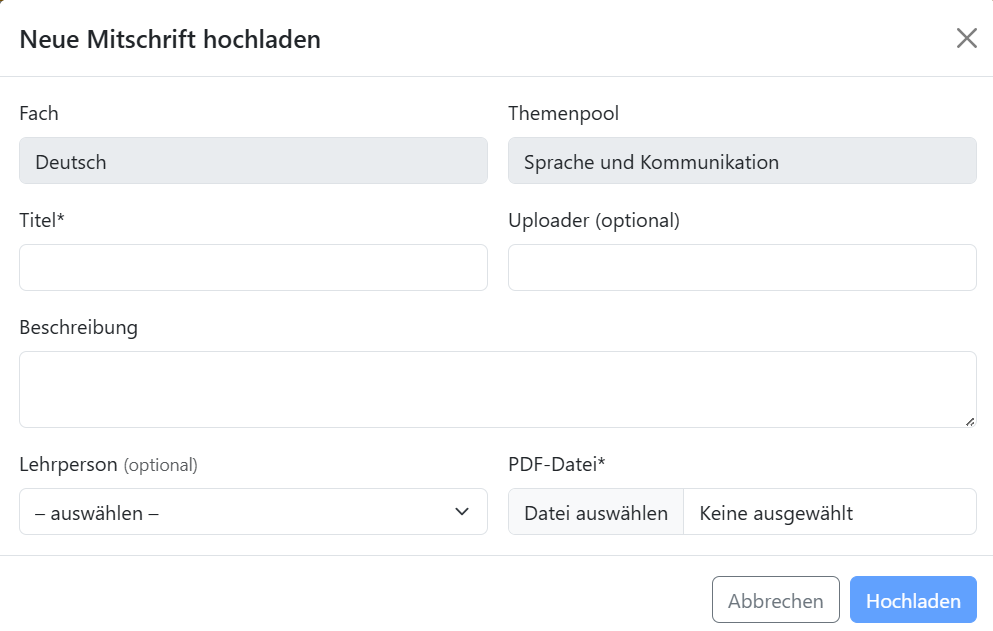
\includegraphics[width=0.7\textwidth]{pics/ab5.png}
    \caption{Mitschriften-Upload-Formular}
    \label{fig:mitschriften-upload}
\end{figure}

\paragraph{Upload als Schüler:in}

Schüler:innen können eigene Mitschriften hochladen. Solange die Mitschrift noch
nicht freigegeben ist, wird sie ausgegraut dargestellt und ist nur für den/die
Ersteller:in sichtbar. In diesem Zustand können Schüler:innen ihre Mitschrift
bearbeiten oder ändern. Nach der Freigabe ist die Mitschrift öffentlich sichtbar;
ab diesem Zeitpunkt können Schüler:innen ausschließlich ihre eigenen
Mitschriften löschen.

\paragraph{Upload als Lehrkraft und Administrator:in}

Lehrkräfte und Administrator:innen können Mitschriften hochladen, die sofort
öffentlich sichtbar sind. Für diese Rolle ist kein Freigabeprozess erforderlich.
Zusätzlich können sie sämtliche Mitschriften – unabhängig vom Ersteller –
bearbeiten oder löschen. Dadurch verfügen sie über die volle Kontrolle über alle
Inhalte innerhalb der Plattform.
